\chapter{Алгоритм на основе восходящего анализа}\label{chpt:GLR}

В данном разделе будут рассмотрены алгоритмы восходящего синтаксического анализа LR-семейсва, в том числе Generalized LR (GLR). Также будет рассмотрено обощение алгоритма GLR для решения задачи поиска путей с контекстно-свободными ограничениями в графах.

\section{Восходящий синтаксический анализ}

Существует большое семейство LR(k) алгоритмов --- алгоритм восходящего синтаксического анализа.
Основная идея, лежащая в основе семейства, заключается в следующем: входная последовательность символов считывается слева направо с попутным добавлением в стек и выполнением сворачивания на стеке --- замены последовательности терминалов и нетерминалов, лежащих наверху стека, на нетерминал, если существует соответствующее правило в исходной грамматике.

Как и в случае с LL используется магазинный автомат, управляемый таблицами, построенными по грамматике.
При этом, у LR анализатора есть два типа команд:
\begin{enumerate}
	\item shift --- прочитать следующий символ входной последовательности, положив его в стек, и перейти в следующее состояние;
	\item reduce(k) --- применить k-ое правило грамматики, правая часть которого уже лежит на стеке: снимаем со стека правую часть продукции и кладём левую часть.
\end{enumerate}

А управляющая таблица выглядит следующим образом.

\begin{center}
  \begin{tabular}{c||c|c|c|c|c||c|c|c|c}
     States & $t_0$   &$\dots$ & $t_a$   & $\dots$ & \$      & $N_0$   &$\dots$ & $N_b$   & $\dots$  \\ \hline \hline
    $\dots$ & $\dots$ &$\dots$ & $\dots$ & $\dots$ & $\dots$ & $\dots$ &$\dots$ & $\dots$ & $\dots$  \\ \hline
    $10$    & $\dots$ &$\dots$ & $s_i$   & $\dots$ & $r_k$   & $\dots$ &$\dots$ & $j$     & $\dots$ \\ \hline
    $\dots$ & $\dots$ &$\dots$ & $\dots$ & $\dots$ & $acc$ & $\dots$ &$\dots$ & $\dots$ & $\dots$
  \end{tabular}
\end{center}

Здесь
\begin{itemize}
  \item $s_i$~--- shift: перенести соответствующи символ в стек и перейти в состояние $i$.
  \item $r_k$~--- reduce(k): в стеке накопилась правая часть продукции $k$, пора производить свёртку.
  \item $j$~--- goto: выполняется после reduce. Сама по себе команда reduce не переводит автомат в новое состояние. Команда goto переведёт автомат в состояние $j$.
  \item $acc$~--- accept: разбор завершился успешно.
\end{itemize}

Если ячейка пустая и в процессе работы мы пропали в неё --- значит произошла ошибка. Для детерминированной работы анализатора требуется, чтобы в каждой ячейке было не более одной команды. Есди это не так, то говорят о возникновении конфликтов.

\begin{itemize}
\item shift-reduce --- ситуация, когда не понятно, читать ли следующий символ или выполнить reduce. Например, если правая часть одного из правил является префиксом правой части другого правила: $N \rightarrow w, M \rightarrow ww'$.
\item reduce-reduce --- ситуация, когда не понятно, к какому правилу нужно применить reduce. Например, если есть два правила с одинаковыми правыми частями: $N \rightarrow w, M \rightarrow w$.
\end{itemize}

Принцип работы LR анализаторов следующий. Пусть у нас есть входная строка, LR-автомат со стеком и управляющая таблица.
В начальный момент на стеке лежит стартовое состояние LR-автомата, позиция во входной строке соответствует её началу.
На каждом шаге анализируется текущий символ входа и текущее состояние, в котором находится автомат, и совершается одно из действий:
\begin{itemize}
\item Если в управляющей таблице нет инструкции для текущего состояния автомата и текущего символа на входе, то завершаем разбор с ошибкой.
\item Иначе выполняем одну из инструкций:
\begin{itemize}
\item в случае acc --- успешно завершаем разбор.
\item в случае shift --- кладем на стек текущий символ входа, сдвигая при этом текущую позицию, и номер нового состояния. Переходим в новое состояние.
\item в случае reduce(k) --- снимаем со стека 2l элементов: l состояний и l терминалов/нетерминалов (где l --- длина правой части k-ого правила), кладём на стек нетерминал левой части правила. Тперь на вершине стека у нас нетерминал $N_a$, а следующий элемент --- состяние $i$. Если в ячейке $(i,N_a)$ управляющей таблицы лежит состояние $j$, то кладём его на вершину стека. Иначе завершаемся с ошибкой.
\end{itemize}
\end{itemize}


Разные алгоритмы из LR-семейсва строят таблицы разными способами и, соответсвенно, могут избегать тех или иных конфликтов. Рассмотрим некорых представителей.

\subsection{LR(0) алгоритм}

Данный алгоритм самый ``слабый'' из семейства --- разбирает наименьший класс языков.
Для построения используются LR(0) пункты.

\begin{definition}
LR(0) пункт (LR(0) item) --- правило грамматики, в правой части которого имеется точка, отделяющая уже разобранную часть правила (слева от точки) от того, что еще предстоит распознать (справа от точки): $A \to \alpha \cdot \beta$, где $A \to \alpha \beta$~--- правило грамматики.
\qed
\end{definition}

Состояние LR(0) автомата --- множество LR(0) пунктов. Для того чтобы изх построить используется операция \textit{closure} или \textit{замыкание}.

\begin{definition}
$closure(X)  = closure(X \cup \{M \rightarrow \cdot \gamma \mid N_i \rightarrow \alpha\cdot M\beta \in X \})$
\qed
\end{definition}

\begin{definition}
Ядро --- исходное множество пунктов, до применения к нему замыкания.
\qed
\end{definition}

Для перемещения точки в пункте используется функция \textit{goto}.

\begin{definition}
$goto(X,p)  = \{N_j \rightarrow \alpha p \cdot \beta \mid N_j \rightarrow \alpha\cdot p\beta \in X \}$
\qed
\end{definition}

Теперь мы можем построить LR(0) автомат.
Первым шагом необходимо расширить грамматику: добавить к исходной грамматике правило вида $S' \to S \$$, где $S$ --- стартовый нетерминал исходной грамматики, $S'$ --- новый стартовый нетерминал (не использовался ранее в грамматике), $\$$ --- маркер конца строки (не входил в терминальный алфавит исходной грамматики).

Далее строим автомат по следующим принципам.

\begin{itemize}
    \item Состояния~--- множества пунктов.
    \item Переходы между состяниями осуществляются по символам грамматики.
    \item Начальное состояние~--- $closure(\{S'\to
    \cdot S \$\})$.
    \item Следующее состояние по текущему состоянию $X$ и смволу $p$ вычисляются как $closure(goto(X, p))$
  \end{itemize}

Управляющая таблица по автомату строится следующим образом.

\begin{itemize}
    \item $acc$ в ячейку, соответствующую финальному состоянию и \$
    \item $s_i$ в ячейку $(j,t)$, если в автомате есть переход из состояния $j$ по терминалу $t$ в состояние $i$
    \item $i$ в ячейку $(j, N)$, если в автомате есть переход из состояния $j$ по нетерминалу $N$ в состояние $i$
    \item $r_k$ в ячейку $(j,t)$, если в состоянии $j$ есть пункт $A \to \alpha \cdot$, где $A \to \alpha$~--- $k$-ое правило грамматики, $t$~--- терминал грамматики
  \end{itemize}

\subsection{SLR(1) алгоритм}

SLR(1) анализатор отличается от LR(0) анализатора построением таблицы по автомату (автомат в точности как у LR(0).
А именно, $r_k$ добавляется в ячейку $(j,t)$, если в состоянии $j$ есть пункт $A \to \alpha \cdot$, где $A \to \alpha$~--- $k$-ое правило грамматики, $t \in FOLLOW(A)$

\subsection{CLR(1) алгоритм}

Canonical LR(1), он же LR(1).
Данный алгоритм является дальнейшим расширением SLR(1): к пунктам добавляются множества предпросмотра (lookahead).

\begin{definition}
Множество предпросмотра для правила $P$ --- терминалы, которые должны встретиться в выведенной строке сразу после строки, выводимой из данного правила.
\qed
\end{definition}

\begin{definition}
CLR пункт: $ [A \to \alpha \cdot \beta, \{ t_0, \dots, t_n\}] $,
где $t_0, \dots, t_n$ --- множество пердпросмотра для правила $A \to \alpha \beta$.
\qed
\end{definition}


\begin{definition}
Пусть дана грамматика $G = \langle \Sigma, N, R, S\rangle$.
\begin{align*}
 closure(X) = closure(X \cup \{&[B \to \cdot \delta, \{FIRST(\beta t_0), \dots, FIRST(\beta t_n)\}] \\
                               &\mid B \to \beta \in R, [A \to \alpha \cdot B \beta, \{t_0, \dots, t_n\}] \in closure(X)\})
\end{align*}
\qed
\end{definition}

Функция \textit{goto} определяется аналогично LR(0), автомат строится по тем же принципам.

При построении управляющей таблицы усиливается правило добавлеия команды \textit{redice}.
А именно, добавляем $r_k$ в ячейку $(j,t_i)$, если в состоянии $j$ есть пункт $[A \to \alpha \cdot, \{t_0, \dots, t_n\}]$, где $A \to \alpha$~--- $k$-ое правило грамматики.

\subsection{Примеры}

Расмотрим построение автоматов и таблиц для различных модефикаций LR алгоритма.

Возьмем следующую грамматику:
\begin{align*}
0)&  S & \rightarrow a S b S \\
1)&  S & \rightarrow \varepsilon
\end{align*}

Расширим вышеупомянутую грамматику, добавив новый стартовый нетерминал S', и далее будем работать с этой расширенной грамматикой:
\begin{align*}
0)&  & S \rightarrow a S b S \\
1)&  & S \rightarrow \varepsilon \\
2)&  & S' \rightarrow S \$
\end{align*}


\begin{example}
Пример ядра и замыкания.

Возьмем правило 2 нашей грамматики, предположим, что мы только начинаем разбирать данное правило.

Ядром в таком случае является item исходного правила: $S' \rightarrow \cdot S \$$

При замыкании добавятся ещё два item'a с правилами по выводу нетерминала 'S', поэтому получаем три item'a: $S' \rightarrow \cdot S\$$, $S \rightarrow \cdot aSbS$ и $S \rightarrow \cdot \varepsilon$
\end{example}

\begin{example}
Пример построения LR(0)-автомата для нашей грамматики с применением замыкания.
\begin{enumerate}
\item Добавляем стартовое состояние: item правила 0 и его замыкание (вместо item'a $S \rightarrow .\varepsilon$ будем писать $S \rightarrow .$).

\begin{tikzpicture}[> = stealth,node distance=3.25cm, on grid, scale=0.8, every node/.style={scale=0.8}]
  \node[r_state] (s_0)
  {
    $
    \begin{aligned}
      S' &\to \cdot S \$ \\
      S  &\to \cdot a S b S \\
      S  &\to \cdot
    \end{aligned}
    $
  };

  \node[num_state] at (s_0.north west) {0};
\end{tikzpicture}

\item По 'S' добавляем переход из стартового состояния в новое состояние 1.

\begin{tikzpicture}[> = stealth,node distance=3.25cm, on grid, scale=0.8, every node/.style={scale=0.8}]
  \node[draw=none, fill=none] at (-1.4, 1.2)  {0};
  \node[draw=none, fill=none] at (3.1, 0.55)  {1};
  \node[r_state] (s_0)
  {
    $
    \begin{aligned}
      S' &\to \cdot S \$ \\
      S  &\to \cdot a S b S \\
      S  &\to \cdot
    \end{aligned}
    $
  };
  \node[r_state] (s_1) [right=of s_0]
  {
    $ S' \to S \cdot \$ $
  };

  \path[->]
    (s_0) edge [above]                node {$S$}  (s_1)
    ;
\end{tikzpicture}

\item По '\$' добавляем переход из состояния 1 в новое состояние 2.

\begin{tikzpicture}[> = stealth,node distance=3.25cm, on grid, scale=0.8, every node/.style={scale=0.8}]
  \node[r_state] (s_0)
  {
    $
    \begin{aligned}
      S' &\to \cdot S \$ \\
      S  &\to \cdot a S b S \\
      S  &\to \cdot
    \end{aligned}
    $
  };
  \node[r_state] (s_1) [right=of s_0]
  {
    $ S' \to S \cdot \$ $
  };
  \node[r_state] (s_2) [right=of s_1]
  {
    $ S' \to S \$ \cdot $
  };

  \node[num_state] at (s_0.north west) {0};
  \node[num_state] at (s_1.north west) {1};
  \node[num_state] at (s_2.north west) {2};

  \path[->]
    (s_0) edge [above]                node {$S$}  (s_1)
    (s_1) edge [above]                node {$\$$} (s_2)
    ;
\end{tikzpicture}

\item По 'a' добавляем переход из стартового состояния в новое состояние 3 и делаем его замыкание. Также добавляем переход по 'a' из этого состояния в себя же.

\begin{tikzpicture}[]
  \node[state] (q_0) {S, 0};
  \node[state] (q_1) [right=of q_0] {S, 1};

  \path[->]
    (q_0) edge[loop above] node {$S \to S \cdot S S$}
                           node[below] {1} ()
          edge[loop below] node {$S \to S \cdot S$}
                           node[above] {2} ()
    (q_1) edge[bend right] node[above] {$S \to S S \cdot S$}
                           node[below] {3} (q_0)
    ;
\end{tikzpicture}

\item По 'S' добавляем переход из состояния 3 в новое состояние 4.

\begin{tikzpicture}[]
  \node[state] (q_0) {S, 0};
  \node[state] (q_1) [right=of q_0] {S, 1};

  \path[->]
    (q_0) edge[loop above] node {$S \to S \cdot S S$}
                           node[below] {1} ()
          edge[loop below] node {$S \to S \cdot S$}
                           node[above] {2} ()
    (q_1) edge[bend left] node[below] {$S \to S S \cdot$}
                          node[above] {4} (q_0)
          edge[bend right] node[above] {$S \to S S \cdot S$}
                           node[below] {3} (q_0)
    ;
\end{tikzpicture}

\item По 'b' добавляем переход из состояния 4 в новое состояние 5 и делаем его замыкание. Также добавляем переход по 'a' из этого состояния в состояние 3.

\begin{tikzpicture}[> = stealth,node distance=3.25cm, on grid, scale=0.8, every node/.style={scale=0.8}]
  \node[draw=none, fill=none] at (-1.4, 1.2)  {0};
  \node[draw=none, fill=none] at (3.1, 0.55)  {1};
  \node[draw=none, fill=none] at (7.1, 0.55)  {2};
  \node[draw=none, fill=none] at (-1.4, -1.8) {3};
  \node[draw=none, fill=none] at (2.9, -2.5)  {4};
  \node[draw=none, fill=none] at (6.7, -1.8)  {5};
  \node[r_state] (s_0)
  {
    $
    \begin{aligned}
      S' &\to \cdot S \$ \\
      S  &\to \cdot a S b S \\
      S  &\to \cdot
    \end{aligned}
    $
  };
  \node[r_state] (s_1) [right=of s_0]
  {
    $ S' \to S \cdot \$ $
  };
  \node[r_state] (s_2) [right=of s_1]
  {
    $ S' \to S \$ \cdot $
  };
  \node[r_state] (s_3) [below=2.5cm of s_0]
  {
    $
    \begin{aligned}
      S  &\to a \cdot S b S \\
      S  &\to \cdot a S b S \\
      S  &\to \cdot
    \end{aligned}
    $
  };
  \node[r_state] (s_4) [right=of s_3]
  {
    $ S \to a S \cdot b S$
  };
  \node[r_state] (s_5) [right=of s_4]
  {
    $
    \begin{aligned}
      S  &\to a S b \cdot S \\
      S  &\to \cdot a S b S \\
      S  &\to \cdot
    \end{aligned}
    $
  };

  \path[->]
    (s_0) edge [left]                 node {$a$}  (s_3)
          edge [above]                node {$S$}  (s_1)
    (s_1) edge [above]                node {$\$$} (s_2)
    (s_3) edge [above]                node {$S$}  (s_4)
          edge [loop below]           node {$a$}  ()
    (s_4) edge [above]                node {$b$}  (s_5)
    (s_5) edge [above, bend right=20] node {$a$}  (s_3)
    ;
\end{tikzpicture}


\item По 'S' добавляем переход из состояния 5 в новое состояние 6. Завершаем построение LR-автомата.

\begin{tikzpicture}[> = stealth,node distance=3.25cm, on grid, scale=0.8, every node/.style={scale=0.8}]
  \node[draw=none, fill=none] at (-1.4, 1.2)  {0};
  \node[draw=none, fill=none] at (3.1, 0.55)  {1};
  \node[draw=none, fill=none] at (7.1, 0.55)  {2};
  \node[draw=none, fill=none] at (-1.4, -1.8) {3};
  \node[draw=none, fill=none] at (2.9, -2.5)  {4};
  \node[draw=none, fill=none] at (6.7, -1.8)  {5};
  \node[draw=none, fill=none] at (11, -2.5)   {6};
  \node[r_state] (s_0)
  {
    $
    \begin{aligned}
      S' &\to \cdot S \$ \\
      S  &\to \cdot a S b S \\
      S  &\to \cdot
    \end{aligned}
    $
  };
  \node[r_state] (s_1) [right=of s_0]
  {
    $ S' \to S \cdot \$ $
  };
  \node[r_state] (s_2) [right=of s_1]
  {
    $ S' \to S \$ \cdot $
  };
  \node[r_state] (s_3) [below=2.5cm of s_0]
  {
    $
    \begin{aligned}
      S  &\to a \cdot S b S \\
      S  &\to \cdot a S b S \\
      S  &\to \cdot
    \end{aligned}
    $
  };
  \node[r_state] (s_4) [right=of s_3]
  {
    $ S \to a S \cdot b S$
  };
  \node[r_state] (s_5) [right=of s_4]
  {
    $
    \begin{aligned}
      S  &\to a S b \cdot S \\
      S  &\to \cdot a S b S \\
      S  &\to \cdot
    \end{aligned}
    $
  };
  \node[r_state] (s_6) [right=of s_5]
  {
    $ S \to a S b S \cdot$
  };

  \path[->]
    (s_0) edge [left]                 node {$a$}  (s_3)
          edge [above]                node {$S$}  (s_1)
    (s_1) edge [above]                node {$\$$} (s_2)
    (s_3) edge [above]                node {$S$}  (s_4)
          edge [loop below]           node {$a$}  ()
    (s_4) edge [above]                node {$b$}  (s_5)
    (s_5) edge [above]                node {$S$}  (s_6)
          edge [above, bend right=20] node {$a$}  (s_3)
    ;
\end{tikzpicture}

\end{enumerate}
\end{example}

Далее будем использовать этот автомат для построения управляющей таблицы.

\begin{example}
Пример управляющей LR(0) таблицы.

\begin{tabular}{c||c|c|c||c}
             & a            & b   & \$  & S \\ \hline
    \hline 0 & $s_3$, $r_1$ & $r_1$ & $r_1$ & 1 \\
    \hline 1 &              &       & acc   &   \\
    \hline 2 & $r_2$        & $r_2$ & $r_2$ &   \\
    \hline 3 & $s_3$, $r_1$ & $r_1$ & $r_1$ & 4 \\
    \hline 4 &              & $s_5$ &       &   \\
    \hline 5 & $s_3, r_1$   & $r_1$ & $r_1$ & 6 \\
    \hline 6 & $r_0$        & $r_0$ & $r_0$ &

\end{tabular}

Как видим, в данном случае в таблице присутствуют shift-reduce конфликты. В случае, когда не удаётся построить таблицу без конфликтов, говорят, что грамматика не LR(0).

\qed
\end{example}


\begin{example}
Пример управляющей LR(1) таблицы. Автомат тот же, однако команды \textit{reduce} расставляются с использованием FOLLOW.

$$
\textit{FOLLOW}_1(S) = \{b, \$\}
$$

\begin{tabular}{c||c|c|c||c}
             & a        & b     & \$    & S \\ \hline
    \hline 0 & $s_3$    & $r_1$ & $r_1$ & 1 \\
    \hline 1 &          &       & acc   &   \\
    \hline 2 &          &       &       &   \\
    \hline 3 & $s_3$    & $r_1$ & $r_1$ & 4 \\
    \hline 4 &          & $s_5$ &       &   \\
    \hline 5 & $s_3$    & $r_1$ & $r_1$ & 6 \\
    \hline 6 &          & $r_0$ & $r_0$ &   \\ [1ex]
\end{tabular}

В данном случае в таблице отсутствуют shift-reduce конфликты. То есть наша грамматика SLR(1), но не LR(0).

\qed
\end{example}

\begin{example}
Пример LR-разбора входного слова abab\$ из языка нашей грамматики с использованием построенных ранее LR-автомата и управляющей таблицы.
\begin{enumerate}
\item Начало разбора. На стеке --- стартовое состояние 0. \\ \\
Вход: \,
\begin{tabular}[c]{ |c|c|c|c|c| }
    \hline \textcolor{red}{a} & b & a & b & \$ \\ \hline
\end{tabular} \\
Стек: \,
\begin{tabular}[c]{ |c|c }
    \hline 0 & \\ \hline
\end{tabular}
\\
\item Выполняем shift 3: сдвигаем указатель на входе, кладем на стек 'a', новое состояние 3 и переходим в него. \\ \\
Вход: \,
\begin{tabular}[c]{ |c|c|c|c|c| }
    \hline a & \textcolor{red}{b} & a & b & \$ \\ \hline
\end{tabular} \\
Стек: \,
\begin{tabular}[c]{ |c|c|c|c }
    \hline 0 & a & 3 & \\ \hline
\end{tabular}
\\
\item Выполняем reduce 1 (кладем на стек 'S'), кладем новое состояние 4 и переходим в него. \\ \\
Вход: \,
\begin{tabular}[c]{ |c|c|c|c|c| }
    \hline a & \textcolor{red}{b} & a & b & \$ \\ \hline
\end{tabular} \\
Стек: \,
\begin{tabular}[c]{ |c|c|c|c|c|c }
    \hline 0 & a & 3 & S & 4 & \\ \hline
\end{tabular}
\\
\item Выполняем shift 5: сдвигаем указатель на входе, кладем на стек 'b', новое состояние 5 и переходим в него. \\ \\
Вход: \,
\begin{tabular}[c]{ |c|c|c|c|c| }
    \hline a & b & \textcolor{red}{a} & b & \$ \\ \hline
\end{tabular}\\
Стек: \,
\begin{tabular}[c]{ |c|c|c|c|c|c|c|c }
    \hline 0 & a & 3 & S & 4 & b & 5 & \\ \hline
\end{tabular}
\\
\item Выполняем shift 3. \\ \\
Вход: \,
\begin{tabular}[c]{ |c|c|c|c|c| }
    \hline a & b & a & \textcolor{red}{b} & \$ \\ \hline
\end{tabular} \\
Стек: \,
\begin{tabular}[c]{ |c|c|c|c|c|c|c|c|c|c }
    \hline 0 & a & 3 & S & 4 & b & 5 & a & 3 & \\ \hline
\end{tabular}
\\
\item Выполняем reduce 1, кладем новое состояние 4 и переходим в него. \\ \\
Вход: \,
\begin{tabular}[c]{ |c|c|c|c|c| }
    \hline a & b & a & \textcolor{red}{b} & \$ \\ \hline
\end{tabular}\\
Стек: \,
\begin{tabular}[c]{ |c|c|c|c|c|c|c|c|c|c|c|c }
    \hline 0 & a & 3 & S & 4 & b & 5 & a & 3 & S & 4 & \\ \hline
\end{tabular}
\\
\item Выполняем shift 5. \\ \\
Вход: \,
\begin{tabular}[c]{ |c|c|c|c|c| }
    \hline a & b & a & b & \textcolor{red}{\$} \\ \hline
\end{tabular} \\
Стек: \,
\begin{tabular}[c]{ |c|c|c|c|c|c|c|c|c|c|c|c|c|c }
    \hline 0 & a & 3 & S & 4 & b & 5 & a & 3 & S & 4 & b & 5 & \\ \hline
\end{tabular}
\\
\item Выполняем reduce 1, кладем новое состояние 6 и переходим в него. \\ \\
Вход: \,
\begin{tabular}[c]{ |c|c|c|c|c| }
    \hline a & b & a & b & \textcolor{red}{\$} \\ \hline
\end{tabular} \\
Стек: \,
\begin{tabular}[c]{ |c|c|c|c|c|c|c|c|c|c|c|c|c|c|c|c }
    \hline 0 & a & 3 & S & 4 & b & 5 & a & 3 & S & 4 & b & 5 & S & 6 & \\ \hline
\end{tabular}
\\
\item Выполняем reduce 0 (снимаем со стека 8 элементов и кладем 'S'), оказываемся в состоянии 5 и делаем переход в новое состояние 6 с добавлением его на стек. \\ \\
Вход: \,
\begin{tabular}[c]{ |c|c|c|c|c| }
    \hline a & b & a & b & \textcolor{red}{\$} \\ \hline
\end{tabular}\\
Стек: \,
\begin{tabular}[c]{ |c|c|c|c|c|c|c|c|c|c }
    \hline 0 & a & 3 & S & 4 & b & 5 & S & 6 & \\ \hline
\end{tabular}
\\
\item Снова выполняем reduce 0, оказываемся в состоянии 0 и делаем переход в новое состояние 1 с добавлением его на стек. Заканчиваем разбор. \\ \\
Вход: \,
\begin{tabular}[c]{ |c|c|c|c|c| }
    \hline a & b & a & b & \textcolor{red}{\$} \\ \hline
\end{tabular} \\
Стек: \,
\begin{tabular}[c]{ |c|c|c|c }
    \hline 0 & S & 1 & \\ \hline
\end{tabular}
\end{enumerate}
\qed
\end{example}

\begin{example}
Пример CLR автомата.

\begin{center}
  \begin{tikzpicture}[> = stealth,node distance=3.25cm, on grid, scale=0.8, every node/.style={scale=0.8}]
  \node[r_state] (s_0)
  {
    $
    \begin{aligned}
      S' &\to \cdot S, \{\$\}  \\
      S  &\to \cdot a S b S, \{\$\} \\
      S  &\to \cdot, \{\$\}
    \end{aligned}
    $
  };
  \node[r_state] (s_1) [below=2.5cm of s_0]
  {
    $
    \begin{aligned}
      S  &\to a \cdot S b S, \{\$\} \\
      S  &\to \cdot a S b S, \{b\} \\
      S  &\to \cdot, \{b\}
    \end{aligned}
    $
  };
  \node[r_state] (s_2) [below=2.5cm of s_1]
  {
    $
    \begin{aligned}
      S  &\to a \cdot S b S, \{b\} \\
      S  &\to \cdot a S b S, \{b\} \\
      S  &\to \cdot, \{b\}
    \end{aligned}
    $
  };
  \node[r_state] (s_3) [right=of s_0]
  {
    $ S' \to S \cdot, \{\$\} $
  };
  \node[r_state] (s_4) [right=of s_1]
  {
    $ S \to a S \cdot b S, \{\$\} $
  };
  \node[r_state] (s_5) [right=of s_2]
  {
    $ S \to a S \cdot b S, \{b\} $
  };
  \node[r_state] (s_6) [right=of s_4]
  {
    $
    \begin{aligned}
      S  &\to a S b \cdot S, \{\$\} \\
      S  &\to \cdot a S b S, \{\$\} \\
      S  &\to \cdot, \{\$\}
    \end{aligned}
    $
  };
  \node[r_state] (s_7) [right=of s_5]
  {
    $
    \begin{aligned}
      S  &\to a S b \cdot S, \{b\} \\
      S  &\to \cdot a S b S, \{b\} \\
      S  &\to \cdot , \{b\}
    \end{aligned}
    $
  };
  \node[r_state] (s_8) [right=of s_6]
  {
    $ S \to a S b S \cdot, \{\$\} $
  };
  \node[r_state] (s_9) [right=of s_7]
  {
    $ S \to a S b S \cdot, \{b\} $
  };

  \node[num_state] at (s_0.north west) {0};
  \node[num_state] at (s_1.north west) {1};
  \node[num_state] at (s_2.north west) {2};
  \node[num_state] at (s_3.north west) {3};
  \node[num_state] at (s_4.north west) {4};
  \node[num_state] at (s_5.north west) {5};
  \node[num_state] at (s_6.north west) {6};
  \node[num_state] at (s_7.north west) {7};
  \node[num_state] at (s_8.north west) {8};
  \node[num_state] at (s_9.north west) {9};


  \path[->]
    (s_0) edge [left]                 node {$a$} (s_1)
          edge [above]                node {$S$} (s_3)
    (s_1) edge [left]                 node {$a$} (s_2)
          edge [above]                node {$S$} (s_4)
    (s_2) edge [loop below]           node {$a$} ()
          edge [above]                node {$S$} (s_5)
    (s_4) edge [above]                node {$b$} (s_6)
    (s_5) edge [above]                node {$b$} (s_7)
    (s_6) edge [above]                node {$S$} (s_8)
          edge [above, bend right=20] node {$a$} (s_1)
    (s_7) edge [above]                node {$S$} (s_9)
          edge [below, bend left=20]  node {$a$} (s_2)
    ;
\end{tikzpicture}
\end{center}
\qed
\end{example}


Существуют и другие модификации, например LALR(1)

На практике конфликты стараются решать ещё и на этапе генерации.
Прикладные инструменты могут сгенерировать парсер по неоднозначной грамматике: из переноса или свёртки выбирать перенос, из нескольких свёрток --- первую в каком-то порядке (обычно в порядке появления соответствующих продукций в грамматике).

\subsection{Сравнение классов LL и LR}

Иерархию языков, распознаваемых различными классами алгоритмов, можно представить следующим  образом.

\begin{center}
  \begin{tikzpicture}
  \node at (0,0) (ll0) {LL(0)};
  \node at (0,3.5) (ll1) {LL(1)};
  \node at (0,4.5) (llk) {LL(k)};
  \node at (3,0) (lr0) {LR(0)};
  \node at (3,1.5) (slr) {SLR(1)};
  \node at (3,2.5) (lalr) {LALR(1)};
  \node at (3,3.5) (clr) {CLR(1)};
  \node at (3,4.5) (lrk) {LR(k)};

  \node[r_state,violet,fit=(ll0)] (a) {};
  \node[draw=none,fit=(a)] (a1) {};
  \node[draw=none,fit=(a1)] (a2) {};
  \node[r_state,violet,fit=(ll0) (ll1) (a)] (b) {};
  \node[r_state,violet,fit=(ll0) (llk) (b)] (c) {};
  \node[r_state,fit=(a2) (lr0)] (d) {};
  \node[r_state,fit=(slr) (d)] (e) {};
  \node[r_state,fit=(lalr) (e)] (f) {};
  \node[r_state,fit=(lalr) (clr) (f) (b)] (g) {};
  \node[r_state,fit=(g) (lalr) (lrk) (c)] (h) {};
\end{tikzpicture}

\end{center}

Из диаграммы видно, что класс языков, распознаваемых LL(k) алгоритмом уже, чем класс языков, распознаваемый LR(k) алгоритмом, при любом конечном $k$. Приведём несколько примеров.
\begin{enumerate}
\item $L = \{a^mb^nc \mid m \geq n \geq 0\} $ является LR(0), но для него не существует LL(1) грамматики.
\item $L = \{ a^n b^n + a^n c^n \mid n > 0\}$ является LR, но не LL.
\item Больше примеров можно найти в работе Джона Битти~\cite{BEATTY1980193}.
\end{enumerate}

\section{GLR и его применение для КС запросов}

Алгоритм LR довольно эффективен, однако позволяет работать не со всеми КС-грамматиками, а только с их подмножеством LR(k). Если грамматика находится за рамками допускаемого класса, некоторые ячейки управляющей таблицы могут содержать несколько значений. В этом случае грамматика отвергалась анализатором.

Чтобы допустить множественные значения в ячейках управляющей таблицы, потребуется некоторый вид недетерминизма, который даст возможность анализатору обрабатывать несколько возможных вариантов синтаксического разбора параллельно. Именно это и предлагает анализатор Generalized LR (GLR)~\cite{tomita-1987-efficient}. Далее мы рассмотрим общий принцип работы, проиллюстрируем его с помощью примера, а также рассмотрим модификации GLR.

\subsection{Классический GLR алгоритм}

Впервые GLR парсер был представлен Масару Томитой в 1987~\cite{tomita-1987-efficient}. В целом, алгоритм работы идентичен LR той разницей, что управляющая таблица модифицирована таким образом, чтобы допускать множественные значения в ячейках. Интерпретатор автомата изменён соответствующим образом.

Для того, чтобы избежать дублирования информации при обработке неоднозначностей, стоит использовать более сложную структуру стека: \textit{граф-структурированный стек} или (\textit{GSS}, Graph Structured Stack). Это направленный граф, в котором вершины соответствуют элементам стека, а ребра их соединяют по правилам управляющей таблицы. У каждой вершины может быть несколько входящих и исходящих дуг: таким образом реализуется то объединение одинаковых состяний и ветвление в случае неоднозначности.

\begin{example}
    \label{glr:example}
    Рассмотрим пример GLR разбора с использованием GSS.

    Возьмем грамматику $G$ следующего вида:
    \begin{align*}
        &0.\quad S' \to S\$ \\
        &1.\quad S \to abC \\
        &2.\quad S \to aBC \\
        &3.\quad B \to b \\
        &4.\quad C \to c
    \end{align*}

    Входное слово $ w $:
    \begin{align*}
        w = abc\$
    \end{align*}

    Построим для данной грамматики LR автомат:

\begin{center}
    \begin{tikzpicture}[> = stealth,node distance=1.25cm, on grid, scale=0.8, every node/.style={scale=0.8}]
  \node[r_state] (s_0)
  {
    $
    \begin{aligned}
      S' &\to \cdot S \$ \\
      S  &\to \cdot a b C \\
      S  &\to \cdot a B C
    \end{aligned}
    $
  };
  \node[r_state] (s_1) [below=2.5cm of s_0]
  {
    $ S' \to S \cdot \$ $
  };
  \node[r_state] (s_acc) [below=2cm of s_1]
  {
    $ S' \to S \$ \cdot $
  };
  \node[r_state] (s_2) [right=3cm of s_0]
  {
    $
    \begin{aligned}
      S  &\to a \cdot B C \\
      S  &\to a \cdot b C \\
      B  &\to \cdot b
    \end{aligned}
    $
  };

  \node[r_state] (s_3) [right=3cm of s_2]
  {
    $
    \begin{aligned}
      S &\to a b \cdot C \\
      B &\to b \cdot \\
      C &\to \cdot c
    \end{aligned}
    $
  };

  \node[r_state] (s_5) [right=3cm of s_3]
  {
    $
    \begin{aligned}
      S &\to a b C \cdot
    \end{aligned}
    $
  };

  \node[r_state] (s_4) [below=2.5cm of s_2]
  {
    $
    \begin{aligned}
      S &\to a B \cdot C \\
      C &\to \cdot c
    \end{aligned}
    $
  };

  \node[r_state] (s_6) [right=3cm of s_4]
  {
    $
    \begin{aligned}
      C &\to c \cdot
    \end{aligned}
    $
  };

  \node[r_state] (s_7) [below=2cm of s_4]
  {
    $
    \begin{aligned}
      S &\to a B C \cdot
    \end{aligned}
    $
  };

  \node[num_state] at (s_0.north west) {0};
  \node[num_state] at (s_1.north west) {1};
  \node[num_state] at (s_2.north west) {2};
  \node[num_state] at (s_3.north west) {3};
  \node[num_state] at (s_4.north west) {4};
  \node[num_state] at (s_5.north west) {5};
  \node[num_state] at (s_6.north west) {6};
  \node[num_state] at (s_7.north west) {7};
  \node[num_state] at (s_acc.north west) {acc};


  \path[->]
    (s_0) edge [above]                node {$a$}  (s_2)
          edge [right]                node {$S$}  (s_1)
    (s_1) edge [right]                node {$\$$} (s_acc)
    (s_2) edge [above]                node {$b$}  (s_3)
          edge [right]                node {$B$}  (s_4)
    (s_3) edge [above]                node {$C$}  (s_5)
          edge [right]                node {$c$}  (s_6)
    (s_4) edge [above]                node {$c$}  (s_6)
          edge [right]                node {$C$}  (s_7)
    ;
\end{tikzpicture}
\end{center}

    И управляющую таблицу:

    \begin{tabular}{c||c|c|c|c||c|c|c}
                 & a     & b     & c            & \$    & B & C & S \\ \hline
        \hline 0 & $s_2$ &       &              &       &   & 1 & \\
        \hline 1 &       &       &              &  acc  &   &   & \\
        \hline 2 &       & $s_3$ &              &       & 4 &   & \\
        \hline 3 &       &       & $s_6$, $r_3$ &       &   & 5 & \\
        \hline 4 &       &       & $s_6$        &       &   & 7 & \\
        \hline 5 &       &       &              & $r_1$ &   &   & \\
        \hline 6 &       &       &              & $r_4$ &   &   & \\
        \hline 7 &       &       &              & $r_2$ &   &   &
    \end{tabular}

    Разберем слово $w$ с помощью алгоритма GLR. Использована следующая аннотация: вершины-состояния обозначены кругами, вершины-символы --- прямоугольниками.
    \begin{enumerate}
        \item Инициализируем GSS стартовым состоянием $v_0$: \\ \\
        Вход: \,
        \begin{tabular}[c]{ |c|c|c|c| }
            \hline a & b & c & \$ \\ \hline
        \end{tabular}
        \qquad GSS: \,
        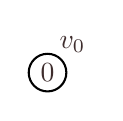
\begin{tikzpicture}[x=0.5pt,y=0.5pt,yscale=-1,xscale=1]
        %uncomment if require: \path (0,306); %set diagram left start at 0, and has height of 306


        % Text Node
        \draw  [line width=0.75]   (92, 109) circle [x radius= 13.6, y radius= 13.6]   ;
        \draw (92,109) node [color={rgb, 255:red, 62; green, 45; blue, 45 }  ,opacity=1 ]  {$0$};
        % Text Node
        \draw (110,89) node [color={rgb, 255:red, 62; green, 45; blue, 45 }  ,opacity=1 ]  {$v_{0}$};


        \end{tikzpicture}
        \\

        \item Видим входной символ '$a$', ищем соответствующую ему операцию в управляющей таблице --- $shift\ 2$, строим новый узел $v_1$: \\ \\
        Вход: \,
        \begin{tabular}[c]{ |c|c|c|c| }
            \hline \textcolor{red}{a} & b & c & \$ \\ \hline
        \end{tabular}
        \qquad GSS: \,
        \begin{tikzpicture}[x=0.5pt,y=0.5pt,yscale=-1,xscale=1]
        %uncomment if require: \path (0,306); %set diagram left start at 0, and has height of 306


        % Text Node
        \draw  [line width=0.75]   (92, 109) circle [x radius= 13.6, y radius= 13.6]   ;
        \draw (92,109) node [color={rgb, 255:red, 62; green, 45; blue, 45 }  ,opacity=1 ]  {$0$};
        % Text Node
        \draw  [line width=0.75]   (138,98) -- (156,98) -- (156,122) -- (138,122) -- cycle  ;
        \draw (147,110) node [scale=1,color={rgb, 255:red, 62; green, 45; blue, 45 }  ,opacity=1 ]  {а};
        % Text Node
        \draw  [line width=0.75]   (203, 110) circle [x radius= 13.6, y radius= 13.6]   ;
        \draw (203,110) node [color={rgb, 255:red, 62; green, 45; blue, 45 }  ,opacity=1 ]  {$2$};
        % Text Node
        \draw (110,89) node [color={rgb, 255:red, 62; green, 45; blue, 45 }  ,opacity=1 ]  {$v_{0}$};
        % Text Node
        \draw (220,89) node [color={rgb, 255:red, 62; green, 45; blue, 45 }  ,opacity=1 ]  {$v_{1}$};
        % Connection
        \draw    (138,109.84) -- (107.6,109.28) ;
        \draw [shift={(105.6,109.25)}, rotate = 361.03999999999996] [color={rgb, 255:red, 0; green, 0; blue, 0 }  ][line width=0.75]    (10.93,-3.29) .. controls (6.95,-1.4) and (3.31,-0.3) .. (0,0) .. controls (3.31,0.3) and (6.95,1.4) .. (10.93,3.29)   ;

        % Connection
        \draw    (189.4,110) -- (158,110) ;
        \draw [shift={(156,110)}, rotate = 360] [color={rgb, 255:red, 0; green, 0; blue, 0 }  ][line width=0.75]    (10.93,-3.29) .. controls (6.95,-1.4) and (3.31,-0.3) .. (0,0) .. controls (3.31,0.3) and (6.95,1.4) .. (10.93,3.29)   ;


        \end{tikzpicture}
        \\

        \item Повторяем для символа '$b$', операции $shift\ 3$ и узла $v_2$: \\ \\
        Вход: \,
        \begin{tabular}[c]{ |c|c|c|c| }
            \hline a & \textcolor{red}{b} & c & \$ \\ \hline
        \end{tabular}
        \qquad GSS: \,
        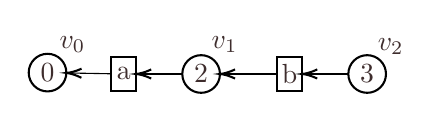
\begin{tikzpicture}[x=0.5pt,y=0.5pt,yscale=-1,xscale=1]
        %uncomment if require: \path (0,306); %set diagram left start at 0, and has height of 306


        % Text Node
        \draw  [line width=0.75]   (92, 109) circle [x radius= 13.6, y radius= 13.6]   ;
        \draw (92,109) node [color={rgb, 255:red, 62; green, 45; blue, 45 }  ,opacity=1 ]  {$0$};
        % Text Node
        \draw  [line width=0.75]   (138,98) -- (156,98) -- (156,122) -- (138,122) -- cycle  ;
        \draw (147,110) node [scale=1,color={rgb, 255:red, 62; green, 45; blue, 45 }  ,opacity=1 ]  {a};
        % Text Node
        \draw  [line width=0.75]   (203, 110) circle [x radius= 13.6, y radius= 13.6]   ;
        \draw (203,110) node [color={rgb, 255:red, 62; green, 45; blue, 45 }  ,opacity=1 ]  {$2$};
        % Text Node
        \draw (110,89) node [color={rgb, 255:red, 62; green, 45; blue, 45 }  ,opacity=1 ]  {$v_{0}$};
        % Text Node
        \draw (220,89) node [color={rgb, 255:red, 62; green, 45; blue, 45 }  ,opacity=1 ]  {$v_{1}$};
        % Text Node
        \draw  [line width=0.75]   (258,98) -- (276,98) -- (276,122) -- (258,122) -- cycle  ;
        \draw (267,110) node [scale=1,color={rgb, 255:red, 62; green, 45; blue, 45 }  ,opacity=1 ]  {b};
        % Text Node
        \draw  [line width=0.75]   (323, 110) circle [x radius= 13.6, y radius= 13.6]   ;
        \draw (323,110) node [color={rgb, 255:red, 62; green, 45; blue, 45 }  ,opacity=1 ]  {$3$};
        % Text Node
        \draw (340,90) node [color={rgb, 255:red, 62; green, 45; blue, 45 }  ,opacity=1 ]  {$v_{2}$};
        % Connection
        \draw    (138,109.84) -- (107.6,109.28) ;
        \draw [shift={(105.6,109.25)}, rotate = 361.03999999999996] [color={rgb, 255:red, 0; green, 0; blue, 0 }  ][line width=0.75]    (10.93,-3.29) .. controls (6.95,-1.4) and (3.31,-0.3) .. (0,0) .. controls (3.31,0.3) and (6.95,1.4) .. (10.93,3.29)   ;

        % Connection
        \draw    (189.4,110) -- (158,110) ;
        \draw [shift={(156,110)}, rotate = 360] [color={rgb, 255:red, 0; green, 0; blue, 0 }  ][line width=0.75]    (10.93,-3.29) .. controls (6.95,-1.4) and (3.31,-0.3) .. (0,0) .. controls (3.31,0.3) and (6.95,1.4) .. (10.93,3.29)   ;

        % Connection
        \draw    (309.4,110) -- (278,110) ;
        \draw [shift={(276,110)}, rotate = 360] [color={rgb, 255:red, 0; green, 0; blue, 0 }  ][line width=0.75]    (10.93,-3.29) .. controls (6.95,-1.4) and (3.31,-0.3) .. (0,0) .. controls (3.31,0.3) and (6.95,1.4) .. (10.93,3.29)   ;

        % Connection
        \draw    (258,110) -- (218.6,110) ;
        \draw [shift={(216.6,110)}, rotate = 360] [color={rgb, 255:red, 0; green, 0; blue, 0 }  ][line width=0.75]    (10.93,-3.29) .. controls (6.95,-1.4) and (3.31,-0.3) .. (0,0) .. controls (3.31,0.3) and (6.95,1.4) .. (10.93,3.29)   ;


        \end{tikzpicture}
        \\

        \item При обработке узла $v_3$ у нас возникает конфликт shift-reduce: $s_6,\ r_3$. Мы смотрим на вершины, смежные $v_2$, на управляющую таблицу и на правило вывода под номером 3 для поиска альтернативного построения стека. Находим $goto\ 4$ и строим вершину $v_3$ с соответствующим переходом по нетерминалу $B$ из $v_1$ (т.к. количество символов в правой части правила вывода 3 равняется 1, значит мы в дереве опустимся на глубину 1 по вершинам-состояниям):\\ \\
        Вход: \,
        \begin{tabular}[c]{ |c|c|c|c| }
            \hline a & b & c & \$ \\ \hline
        \end{tabular}
        \qquad GSS: \,
        \begin{tikzpicture}[x=0.5pt,y=0.5pt,yscale=-1,xscale=1]
        %uncomment if require: \path (0,422); %set diagram left start at 0, and has height of 422


        % Text Node
        \draw  [line width=0.75]   (92, 110) circle [x radius= 13.6, y radius= 13.6]   ;
        \draw (92,110) node [color={rgb, 255:red, 62; green, 45; blue, 45 }  ,opacity=1 ]  {$0$};
        % Text Node
        \draw  [line width=0.75]   (138,98) -- (156,98) -- (156,122) -- (138,122) -- cycle  ;
        \draw (147,110) node [scale=1,color={rgb, 255:red, 62; green, 45; blue, 45 }  ,opacity=1 ]  {а};
        % Text Node
        \draw  [line width=0.75]   (203, 110) circle [x radius= 13.6, y radius= 13.6]   ;
        \draw (203,110) node [color={rgb, 255:red, 62; green, 45; blue, 45 }  ,opacity=1 ]  {$2$};
        % Text Node
        \draw (110,89) node [color={rgb, 255:red, 62; green, 45; blue, 45 }  ,opacity=1 ]  {$v_{0}$};
        % Text Node
        \draw (220,89) node [color={rgb, 255:red, 62; green, 45; blue, 45 }  ,opacity=1 ]  {$v_{1}$};
        % Text Node
        \draw  [line width=0.75]   (258,98) -- (276,98) -- (276,122) -- (258,122) -- cycle  ;
        \draw (267,110) node [scale=1,color={rgb, 255:red, 62; green, 45; blue, 45 }  ,opacity=1 ]  {b};
        % Text Node
        \draw  [line width=0.75]   (323, 110) circle [x radius= 13.6, y radius= 13.6]   ;
        \draw (323,110) node [color={rgb, 255:red, 62; green, 45; blue, 45 }  ,opacity=1 ]  {$3$};
        % Text Node
        \draw (340,90) node [color={rgb, 255:red, 62; green, 45; blue, 45 }  ,opacity=1 ]  {$v_{2}$};
        % Text Node
        \draw  [line width=0.75]   (258,158) -- (276,158) -- (276,182) -- (258,182) -- cycle  ;
        \draw (267,170) node [scale=1,color={rgb, 255:red, 62; green, 45; blue, 45 }  ,opacity=1 ]  {B};
        % Text Node
        \draw  [line width=0.75]   (323, 170) circle [x radius= 13.6, y radius= 13.6]   ;
        \draw (323,170) node [color={rgb, 255:red, 62; green, 45; blue, 45 }  ,opacity=1 ]  {$4$};
        % Text Node
        \draw (340,149) node [color={rgb, 255:red, 62; green, 45; blue, 45 }  ,opacity=1 ]  {$v_{3}$};
        % Connection
        \draw    (138,110) -- (107.6,110) ;
        \draw [shift={(105.6,110)}, rotate = 360] [color={rgb, 255:red, 0; green, 0; blue, 0 }  ][line width=0.75]    (10.93,-3.29) .. controls (6.95,-1.4) and (3.31,-0.3) .. (0,0) .. controls (3.31,0.3) and (6.95,1.4) .. (10.93,3.29)   ;

        % Connection
        \draw    (189.4,110) -- (158,110) ;
        \draw [shift={(156,110)}, rotate = 360] [color={rgb, 255:red, 0; green, 0; blue, 0 }  ][line width=0.75]    (10.93,-3.29) .. controls (6.95,-1.4) and (3.31,-0.3) .. (0,0) .. controls (3.31,0.3) and (6.95,1.4) .. (10.93,3.29)   ;

        % Connection
        \draw    (309.4,110) -- (278,110) ;
        \draw [shift={(276,110)}, rotate = 360] [color={rgb, 255:red, 0; green, 0; blue, 0 }  ][line width=0.75]    (10.93,-3.29) .. controls (6.95,-1.4) and (3.31,-0.3) .. (0,0) .. controls (3.31,0.3) and (6.95,1.4) .. (10.93,3.29)   ;

        % Connection
        \draw    (258,110) -- (218.6,110) ;
        \draw [shift={(216.6,110)}, rotate = 360] [color={rgb, 255:red, 0; green, 0; blue, 0 }  ][line width=0.75]    (10.93,-3.29) .. controls (6.95,-1.4) and (3.31,-0.3) .. (0,0) .. controls (3.31,0.3) and (6.95,1.4) .. (10.93,3.29)   ;

        % Connection
        \draw    (309.4,170) -- (278,170) ;
        \draw [shift={(276,170)}, rotate = 360] [color={rgb, 255:red, 0; green, 0; blue, 0 }  ][line width=0.75]    (10.93,-3.29) .. controls (6.95,-1.4) and (3.31,-0.3) .. (0,0) .. controls (3.31,0.3) and (6.95,1.4) .. (10.93,3.29)   ;

        % Connection
        \draw    (258,168.07) .. controls (230.15,163.58) and (213.3,149.18) .. (207.42,124.89) ;
        \draw [shift={(206.99,123.01)}, rotate = 437.91] [color={rgb, 255:red, 0; green, 0; blue, 0 }  ][line width=0.75]    (10.93,-3.29) .. controls (6.95,-1.4) and (3.31,-0.3) .. (0,0) .. controls (3.31,0.3) and (6.95,1.4) .. (10.93,3.29)   ;


        \end{tikzpicture}
        \\

        \item Читаем символ '$c$' и ищем в управляющей таблице переходы из состояний 3 и 4 (так как узлы $v_2$ и $v_3$ находятся на одном уровне, то есть были построены после чтения одного символа из входного слова). Таким переходом оказывается $s_6$ в обоих случаях, поэтому соединяем узел $v_4$ с обоими рассмотренными узлами:\\ \\
        Вход: \,
        \begin{tabular}[c]{ |c|c|c|c| }
            \hline a & b & \textcolor{red}{c} & \$ \\ \hline
        \end{tabular}
        \qquad GSS: \,
        \begin{tikzpicture}[x=0.5pt,y=0.5pt,yscale=-1,xscale=1]
        %uncomment if require: \path (0,422); %set diagram left start at 0, and has height of 422


        % Text Node
        \draw  [line width=0.75]   (92, 110) circle [x radius= 13.6, y radius= 13.6]   ;
        \draw (92,110) node [color={rgb, 255:red, 62; green, 45; blue, 45 }  ,opacity=1 ]  {$0$};
        % Text Node
        \draw  [line width=0.75]   (138,98) -- (156,98) -- (156,122) -- (138,122) -- cycle  ;
        \draw (147,110) node [scale=1,color={rgb, 255:red, 62; green, 45; blue, 45 }  ,opacity=1 ]  {а};
        % Text Node
        \draw  [line width=0.75]   (203, 110) circle [x radius= 13.6, y radius= 13.6]   ;
        \draw (203,110) node [color={rgb, 255:red, 62; green, 45; blue, 45 }  ,opacity=1 ]  {$2$};
        % Text Node
        \draw (110,89) node [color={rgb, 255:red, 62; green, 45; blue, 45 }  ,opacity=1 ]  {$v_{0}$};
        % Text Node
        \draw (220,89) node [color={rgb, 255:red, 62; green, 45; blue, 45 }  ,opacity=1 ]  {$v_{1}$};
        % Text Node
        \draw  [line width=0.75]   (258,98) -- (276,98) -- (276,122) -- (258,122) -- cycle  ;
        \draw (267,110) node [scale=1,color={rgb, 255:red, 62; green, 45; blue, 45 }  ,opacity=1 ]  {b};
        % Text Node
        \draw  [line width=0.75]   (323, 110) circle [x radius= 13.6, y radius= 13.6]   ;
        \draw (323,110) node [color={rgb, 255:red, 62; green, 45; blue, 45 }  ,opacity=1 ]  {$3$};
        % Text Node
        \draw (340,90) node [color={rgb, 255:red, 62; green, 45; blue, 45 }  ,opacity=1 ]  {$v_{2}$};
        % Text Node
        \draw  [line width=0.75]   (258,158) -- (276,158) -- (276,182) -- (258,182) -- cycle  ;
        \draw (267,170) node [scale=1,color={rgb, 255:red, 62; green, 45; blue, 45 }  ,opacity=1 ]  {B};
        % Text Node
        \draw  [line width=0.75]   (323, 170) circle [x radius= 13.6, y radius= 13.6]   ;
        \draw (323,170) node [color={rgb, 255:red, 62; green, 45; blue, 45 }  ,opacity=1 ]  {$4$};
        % Text Node
        \draw (340,149) node [color={rgb, 255:red, 62; green, 45; blue, 45 }  ,opacity=1 ]  {$v_{3}$};
        % Text Node
        \draw  [line width=0.75]   (374,98) -- (392,98) -- (392,122) -- (374,122) -- cycle  ;
        \draw (383,110) node [scale=1,color={rgb, 255:red, 62; green, 45; blue, 45 }  ,opacity=1 ]  {c};
        % Text Node
        \draw  [line width=0.75]   (374,158) -- (392,158) -- (392,182) -- (374,182) -- cycle  ;
        \draw (383,170) node [scale=1,color={rgb, 255:red, 62; green, 45; blue, 45 }  ,opacity=1 ]  {c};
        % Text Node
        \draw  [line width=0.75]   (437, 110) circle [x radius= 13.6, y radius= 13.6]   ;
        \draw (437,110) node [color={rgb, 255:red, 62; green, 45; blue, 45 }  ,opacity=1 ]  {$6$};
        % Text Node
        \draw (450,89) node [color={rgb, 255:red, 62; green, 45; blue, 45 }  ,opacity=1 ]  {$v_{4}$};
        % Connection
        \draw    (138,110) -- (107.6,110) ;
        \draw [shift={(105.6,110)}, rotate = 360] [color={rgb, 255:red, 0; green, 0; blue, 0 }  ][line width=0.75]    (10.93,-3.29) .. controls (6.95,-1.4) and (3.31,-0.3) .. (0,0) .. controls (3.31,0.3) and (6.95,1.4) .. (10.93,3.29)   ;

        % Connection
        \draw    (189.4,110) -- (158,110) ;
        \draw [shift={(156,110)}, rotate = 360] [color={rgb, 255:red, 0; green, 0; blue, 0 }  ][line width=0.75]    (10.93,-3.29) .. controls (6.95,-1.4) and (3.31,-0.3) .. (0,0) .. controls (3.31,0.3) and (6.95,1.4) .. (10.93,3.29)   ;

        % Connection
        \draw    (309.4,110) -- (278,110) ;
        \draw [shift={(276,110)}, rotate = 360] [color={rgb, 255:red, 0; green, 0; blue, 0 }  ][line width=0.75]    (10.93,-3.29) .. controls (6.95,-1.4) and (3.31,-0.3) .. (0,0) .. controls (3.31,0.3) and (6.95,1.4) .. (10.93,3.29)   ;

        % Connection
        \draw    (258,110) -- (218.6,110) ;
        \draw [shift={(216.6,110)}, rotate = 360] [color={rgb, 255:red, 0; green, 0; blue, 0 }  ][line width=0.75]    (10.93,-3.29) .. controls (6.95,-1.4) and (3.31,-0.3) .. (0,0) .. controls (3.31,0.3) and (6.95,1.4) .. (10.93,3.29)   ;

        % Connection
        \draw    (309.4,170) -- (278,170) ;
        \draw [shift={(276,170)}, rotate = 360] [color={rgb, 255:red, 0; green, 0; blue, 0 }  ][line width=0.75]    (10.93,-3.29) .. controls (6.95,-1.4) and (3.31,-0.3) .. (0,0) .. controls (3.31,0.3) and (6.95,1.4) .. (10.93,3.29)   ;

        % Connection
        \draw    (258,168.07) .. controls (230.15,163.58) and (213.3,149.18) .. (207.42,124.89) ;
        \draw [shift={(206.99,123.01)}, rotate = 437.91] [color={rgb, 255:red, 0; green, 0; blue, 0 }  ][line width=0.75]    (10.93,-3.29) .. controls (6.95,-1.4) and (3.31,-0.3) .. (0,0) .. controls (3.31,0.3) and (6.95,1.4) .. (10.93,3.29)   ;

        % Connection
        \draw    (374,110) -- (338.6,110) ;
        \draw [shift={(336.6,110)}, rotate = 360] [color={rgb, 255:red, 0; green, 0; blue, 0 }  ][line width=0.75]    (10.93,-3.29) .. controls (6.95,-1.4) and (3.31,-0.3) .. (0,0) .. controls (3.31,0.3) and (6.95,1.4) .. (10.93,3.29)   ;

        % Connection
        \draw    (423.4,110) -- (394,110) ;
        \draw [shift={(392,110)}, rotate = 360] [color={rgb, 255:red, 0; green, 0; blue, 0 }  ][line width=0.75]    (10.93,-3.29) .. controls (6.95,-1.4) and (3.31,-0.3) .. (0,0) .. controls (3.31,0.3) and (6.95,1.4) .. (10.93,3.29)   ;

        % Connection
        \draw    (435.82,123.55) .. controls (435.9,150.31) and (416.89,165.24) .. (393.78,168.34) ;
        \draw [shift={(392,168.55)}, rotate = 353.9] [color={rgb, 255:red, 0; green, 0; blue, 0 }  ][line width=0.75]    (10.93,-3.29) .. controls (6.95,-1.4) and (3.31,-0.3) .. (0,0) .. controls (3.31,0.3) and (6.95,1.4) .. (10.93,3.29)   ;

        % Connection
        \draw    (374,170) -- (338.6,170) ;
        \draw [shift={(336.6,170)}, rotate = 360] [color={rgb, 255:red, 0; green, 0; blue, 0 }  ][line width=0.75]    (10.93,-3.29) .. controls (6.95,-1.4) and (3.31,-0.3) .. (0,0) .. controls (3.31,0.3) and (6.95,1.4) .. (10.93,3.29)   ;


        \end{tikzpicture}
        \\

        \item При обработке узла $v_4$ находим соответствующею 6-ому состоянию редукцию по правилу 4. Его правая часть содержит один символ '$c$', 2 вершины-символа с которым достижимы из $v_4$. Находим вершины-состояния, которые смежны с этими вершинами-символами и обрабатываем переходы по левой части правила 4. Такими переходами по нетерминалу $C$ оказываются $5$ и $7$. Строим соответствующие им вершины $v_5$ и $v_6$:\\ \\
        Вход: \,
        \begin{tabular}[c]{ |c|c|c|c| }
            \hline a & b & c & \$ \\ \hline
        \end{tabular}
        \qquad GSS: \,
        \begin{tikzpicture}[x=0.5pt,y=0.5pt,yscale=-1,xscale=1]
        %uncomment if require: \path (0,422); %set diagram left start at 0, and has height of 422


        % Text Node
        \draw  [line width=0.75]   (92, 110) circle [x radius= 13.6, y radius= 13.6]   ;
        \draw (92,110) node [color={rgb, 255:red, 62; green, 45; blue, 45 }  ,opacity=1 ]  {$0$};
        % Text Node
        \draw  [line width=0.75]   (138,98) -- (156,98) -- (156,122) -- (138,122) -- cycle  ;
        \draw (147,110) node [scale=1,color={rgb, 255:red, 62; green, 45; blue, 45 }  ,opacity=1 ]  {а};
        % Text Node
        \draw  [line width=0.75]   (203, 110) circle [x radius= 13.6, y radius= 13.6]   ;
        \draw (203,110) node [color={rgb, 255:red, 62; green, 45; blue, 45 }  ,opacity=1 ]  {$2$};
        % Text Node
        \draw (110,89) node [color={rgb, 255:red, 62; green, 45; blue, 45 }  ,opacity=1 ]  {$v_{0}$};
        % Text Node
        \draw (220,89) node [color={rgb, 255:red, 62; green, 45; blue, 45 }  ,opacity=1 ]  {$v_{1}$};
        % Text Node
        \draw  [line width=0.75]   (258,98) -- (276,98) -- (276,122) -- (258,122) -- cycle  ;
        \draw (267,110) node [scale=1,color={rgb, 255:red, 62; green, 45; blue, 45 }  ,opacity=1 ]  {b};
        % Text Node
        \draw  [line width=0.75]   (323, 110) circle [x radius= 13.6, y radius= 13.6]   ;
        \draw (323,110) node [color={rgb, 255:red, 62; green, 45; blue, 45 }  ,opacity=1 ]  {$3$};
        % Text Node
        \draw (340,90) node [color={rgb, 255:red, 62; green, 45; blue, 45 }  ,opacity=1 ]  {$v_{2}$};
        % Text Node
        \draw  [line width=0.75]   (258,158) -- (276,158) -- (276,182) -- (258,182) -- cycle  ;
        \draw (267,170) node [scale=1,color={rgb, 255:red, 62; green, 45; blue, 45 }  ,opacity=1 ]  {B};
        % Text Node
        \draw  [line width=0.75]   (323, 170) circle [x radius= 13.6, y radius= 13.6]   ;
        \draw (323,170) node [color={rgb, 255:red, 62; green, 45; blue, 45 }  ,opacity=1 ]  {$4$};
        % Text Node
        \draw (340,149) node [color={rgb, 255:red, 62; green, 45; blue, 45 }  ,opacity=1 ]  {$v_{3}$};
        % Text Node
        \draw  [line width=0.75]   (374,98) -- (392,98) -- (392,122) -- (374,122) -- cycle  ;
        \draw (383,110) node [scale=1,color={rgb, 255:red, 62; green, 45; blue, 45 }  ,opacity=1 ]  {c};
        % Text Node
        \draw  [line width=0.75]   (374,158) -- (392,158) -- (392,182) -- (374,182) -- cycle  ;
        \draw (383,170) node [scale=1,color={rgb, 255:red, 62; green, 45; blue, 45 }  ,opacity=1 ]  {c};
        % Text Node
        \draw  [line width=0.75]   (437, 110) circle [x radius= 13.6, y radius= 13.6]   ;
        \draw (437,110) node [color={rgb, 255:red, 62; green, 45; blue, 45 }  ,opacity=1 ]  {$6$};
        % Text Node
        \draw (450,89) node [color={rgb, 255:red, 62; green, 45; blue, 45 }  ,opacity=1 ]  {$v_{4}$};
        % Text Node
        \draw  [line width=0.75]   (372,38) -- (392,38) -- (392,62) -- (372,62) -- cycle  ;
        \draw (382,50) node [scale=1,color={rgb, 255:red, 62; green, 45; blue, 45 }  ,opacity=1 ]  {C};
        % Text Node
        \draw  [line width=0.75]   (372,218) -- (392,218) -- (392,242) -- (372,242) -- cycle  ;
        \draw (382,230) node [scale=1,color={rgb, 255:red, 62; green, 45; blue, 45 }  ,opacity=1 ]  {C};
        % Text Node
        \draw  [line width=0.75]   (437, 50) circle [x radius= 13.6, y radius= 13.6]   ;
        \draw (437,50) node [color={rgb, 255:red, 62; green, 45; blue, 45 }  ,opacity=1 ]  {$5$};
        % Text Node
        \draw  [line width=0.75]   (437, 231) circle [x radius= 13.6, y radius= 13.6]   ;
        \draw (437,231) node [color={rgb, 255:red, 62; green, 45; blue, 45 }  ,opacity=1 ]  {$7$};
        % Text Node
        \draw (452,28) node [color={rgb, 255:red, 62; green, 45; blue, 45 }  ,opacity=1 ]  {$v_{5}$};
        % Text Node
        \draw (452,208) node [color={rgb, 255:red, 62; green, 45; blue, 45 }  ,opacity=1 ]  {$v_{6}$};
        % Connection
        \draw    (138,110) -- (107.6,110) ;
        \draw [shift={(105.6,110)}, rotate = 360] [color={rgb, 255:red, 0; green, 0; blue, 0 }  ][line width=0.75]    (10.93,-3.29) .. controls (6.95,-1.4) and (3.31,-0.3) .. (0,0) .. controls (3.31,0.3) and (6.95,1.4) .. (10.93,3.29)   ;

        % Connection
        \draw    (189.4,110) -- (158,110) ;
        \draw [shift={(156,110)}, rotate = 360] [color={rgb, 255:red, 0; green, 0; blue, 0 }  ][line width=0.75]    (10.93,-3.29) .. controls (6.95,-1.4) and (3.31,-0.3) .. (0,0) .. controls (3.31,0.3) and (6.95,1.4) .. (10.93,3.29)   ;

        % Connection
        \draw    (309.4,110) -- (278,110) ;
        \draw [shift={(276,110)}, rotate = 360] [color={rgb, 255:red, 0; green, 0; blue, 0 }  ][line width=0.75]    (10.93,-3.29) .. controls (6.95,-1.4) and (3.31,-0.3) .. (0,0) .. controls (3.31,0.3) and (6.95,1.4) .. (10.93,3.29)   ;

        % Connection
        \draw    (258,110) -- (218.6,110) ;
        \draw [shift={(216.6,110)}, rotate = 360] [color={rgb, 255:red, 0; green, 0; blue, 0 }  ][line width=0.75]    (10.93,-3.29) .. controls (6.95,-1.4) and (3.31,-0.3) .. (0,0) .. controls (3.31,0.3) and (6.95,1.4) .. (10.93,3.29)   ;

        % Connection
        \draw    (309.4,170) -- (278,170) ;
        \draw [shift={(276,170)}, rotate = 360] [color={rgb, 255:red, 0; green, 0; blue, 0 }  ][line width=0.75]    (10.93,-3.29) .. controls (6.95,-1.4) and (3.31,-0.3) .. (0,0) .. controls (3.31,0.3) and (6.95,1.4) .. (10.93,3.29)   ;

        % Connection
        \draw    (258,168.07) .. controls (230.15,163.58) and (213.3,149.18) .. (207.42,124.89) ;
        \draw [shift={(206.99,123.01)}, rotate = 437.91] [color={rgb, 255:red, 0; green, 0; blue, 0 }  ][line width=0.75]    (10.93,-3.29) .. controls (6.95,-1.4) and (3.31,-0.3) .. (0,0) .. controls (3.31,0.3) and (6.95,1.4) .. (10.93,3.29)   ;

        % Connection
        \draw    (374,110) -- (338.6,110) ;
        \draw [shift={(336.6,110)}, rotate = 360] [color={rgb, 255:red, 0; green, 0; blue, 0 }  ][line width=0.75]    (10.93,-3.29) .. controls (6.95,-1.4) and (3.31,-0.3) .. (0,0) .. controls (3.31,0.3) and (6.95,1.4) .. (10.93,3.29)   ;

        % Connection
        \draw    (423.4,110) -- (394,110) ;
        \draw [shift={(392,110)}, rotate = 360] [color={rgb, 255:red, 0; green, 0; blue, 0 }  ][line width=0.75]    (10.93,-3.29) .. controls (6.95,-1.4) and (3.31,-0.3) .. (0,0) .. controls (3.31,0.3) and (6.95,1.4) .. (10.93,3.29)   ;

        % Connection
        \draw    (435.82,123.55) .. controls (435.9,150.31) and (416.89,165.24) .. (393.78,168.34) ;
        \draw [shift={(392,168.55)}, rotate = 353.9] [color={rgb, 255:red, 0; green, 0; blue, 0 }  ][line width=0.75]    (10.93,-3.29) .. controls (6.95,-1.4) and (3.31,-0.3) .. (0,0) .. controls (3.31,0.3) and (6.95,1.4) .. (10.93,3.29)   ;

        % Connection
        \draw    (374,170) -- (338.6,170) ;
        \draw [shift={(336.6,170)}, rotate = 360] [color={rgb, 255:red, 0; green, 0; blue, 0 }  ][line width=0.75]    (10.93,-3.29) .. controls (6.95,-1.4) and (3.31,-0.3) .. (0,0) .. controls (3.31,0.3) and (6.95,1.4) .. (10.93,3.29)   ;

        % Connection
        \draw    (372,50.52) .. controls (341.88,50.18) and (326.06,64.88) .. (324.53,94.64) ;
        \draw [shift={(324.46,96.48)}, rotate = 271.78] [color={rgb, 255:red, 0; green, 0; blue, 0 }  ][line width=0.75]    (10.93,-3.29) .. controls (6.95,-1.4) and (3.31,-0.3) .. (0,0) .. controls (3.31,0.3) and (6.95,1.4) .. (10.93,3.29)   ;

        % Connection
        \draw    (372,229.65) .. controls (341.88,230.53) and (326.05,215.79) .. (324.5,185.41) ;
        \draw [shift={(324.42,183.53)}, rotate = 448.21] [color={rgb, 255:red, 0; green, 0; blue, 0 }  ][line width=0.75]    (10.93,-3.29) .. controls (6.95,-1.4) and (3.31,-0.3) .. (0,0) .. controls (3.31,0.3) and (6.95,1.4) .. (10.93,3.29)   ;

        % Connection
        \draw    (423.4,50) -- (394,50) ;
        \draw [shift={(392,50)}, rotate = 360] [color={rgb, 255:red, 0; green, 0; blue, 0 }  ][line width=0.75]    (10.93,-3.29) .. controls (6.95,-1.4) and (3.31,-0.3) .. (0,0) .. controls (3.31,0.3) and (6.95,1.4) .. (10.93,3.29)   ;

        % Connection
        \draw    (423.4,230.75) -- (394,230.22) ;
        \draw [shift={(392,230.18)}, rotate = 361.03999999999996] [color={rgb, 255:red, 0; green, 0; blue, 0 }  ][line width=0.75]    (10.93,-3.29) .. controls (6.95,-1.4) and (3.31,-0.3) .. (0,0) .. controls (3.31,0.3) and (6.95,1.4) .. (10.93,3.29)   ;


        \end{tikzpicture}
        \\

        \item При обработке узлов $v_5$ и $v_6$ находим редукции с символом '$S$' в левой части и тремя символами в правой. Возвращаемся на 3 вершины-состояния назад и строим вершину $v_7$ с переходом по $S$: \\ \\
        Вход: \,
        \begin{tabular}[c]{ |c|c|c|c| }
            \hline a & b & c & \$ \\ \hline
        \end{tabular}
        \qquad GSS: \,
        \begin{tikzpicture}[x=0.5pt,y=0.5pt,yscale=-1,xscale=1]
        %uncomment if require: \path (0,422); %set diagram left start at 0, and has height of 422


        % Text Node
        \draw  [line width=0.75]   (92, 110) circle [x radius= 13.6, y radius= 13.6]   ;
        \draw (92,110) node [color={rgb, 255:red, 62; green, 45; blue, 45 }  ,opacity=1 ]  {$0$};
        % Text Node
        \draw  [line width=0.75]   (138,98) -- (156,98) -- (156,122) -- (138,122) -- cycle  ;
        \draw (147,110) node [scale=1,color={rgb, 255:red, 62; green, 45; blue, 45 }  ,opacity=1 ]  {а};
        % Text Node
        \draw  [line width=0.75]   (203, 110) circle [x radius= 13.6, y radius= 13.6]   ;
        \draw (203,110) node [color={rgb, 255:red, 62; green, 45; blue, 45 }  ,opacity=1 ]  {$2$};
        % Text Node
        \draw (110,89) node [color={rgb, 255:red, 62; green, 45; blue, 45 }  ,opacity=1 ]  {$v_{0}$};
        % Text Node
        \draw (220,89) node [color={rgb, 255:red, 62; green, 45; blue, 45 }  ,opacity=1 ]  {$v_{1}$};
        % Text Node
        \draw  [line width=0.75]   (258,98) -- (276,98) -- (276,122) -- (258,122) -- cycle  ;
        \draw (267,110) node [scale=1,color={rgb, 255:red, 62; green, 45; blue, 45 }  ,opacity=1 ]  {b};
        % Text Node
        \draw  [line width=0.75]   (323, 110) circle [x radius= 13.6, y radius= 13.6]   ;
        \draw (323,110) node [color={rgb, 255:red, 62; green, 45; blue, 45 }  ,opacity=1 ]  {$3$};
        % Text Node
        \draw (340,90) node [color={rgb, 255:red, 62; green, 45; blue, 45 }  ,opacity=1 ]  {$v_{2}$};
        % Text Node
        \draw  [line width=0.75]   (258,158) -- (276,158) -- (276,182) -- (258,182) -- cycle  ;
        \draw (267,170) node [scale=1,color={rgb, 255:red, 62; green, 45; blue, 45 }  ,opacity=1 ]  {B};
        % Text Node
        \draw  [line width=0.75]   (323, 170) circle [x radius= 13.6, y radius= 13.6]   ;
        \draw (323,170) node [color={rgb, 255:red, 62; green, 45; blue, 45 }  ,opacity=1 ]  {$4$};
        % Text Node
        \draw (340,149) node [color={rgb, 255:red, 62; green, 45; blue, 45 }  ,opacity=1 ]  {$v_{3}$};
        % Text Node
        \draw  [line width=0.75]   (374,98) -- (392,98) -- (392,122) -- (374,122) -- cycle  ;
        \draw (383,110) node [scale=1,color={rgb, 255:red, 62; green, 45; blue, 45 }  ,opacity=1 ]  {c};
        % Text Node
        \draw  [line width=0.75]   (374,158) -- (392,158) -- (392,182) -- (374,182) -- cycle  ;
        \draw (383,170) node [scale=1,color={rgb, 255:red, 62; green, 45; blue, 45 }  ,opacity=1 ]  {c};
        % Text Node
        \draw  [line width=0.75]   (437, 110) circle [x radius= 13.6, y radius= 13.6]   ;
        \draw (437,110) node [color={rgb, 255:red, 62; green, 45; blue, 45 }  ,opacity=1 ]  {$6$};
        % Text Node
        \draw (450,89) node [color={rgb, 255:red, 62; green, 45; blue, 45 }  ,opacity=1 ]  {$v_{4}$};
        % Text Node
        \draw  [line width=0.75]   (372,38) -- (392,38) -- (392,62) -- (372,62) -- cycle  ;
        \draw (382,50) node [scale=1,color={rgb, 255:red, 62; green, 45; blue, 45 }  ,opacity=1 ]  {C};
        % Text Node
        \draw  [line width=0.75]   (372,218) -- (392,218) -- (392,242) -- (372,242) -- cycle  ;
        \draw (382,230) node [scale=1,color={rgb, 255:red, 62; green, 45; blue, 45 }  ,opacity=1 ]  {C};
        % Text Node
        \draw  [line width=0.75]   (437, 50) circle [x radius= 13.6, y radius= 13.6]   ;
        \draw (437,50) node [color={rgb, 255:red, 62; green, 45; blue, 45 }  ,opacity=1 ]  {$5$};
        % Text Node
        \draw  [line width=0.75]   (437, 231) circle [x radius= 13.6, y radius= 13.6]   ;
        \draw (437,231) node [color={rgb, 255:red, 62; green, 45; blue, 45 }  ,opacity=1 ]  {$7$};
        % Text Node
        \draw (452,28) node [color={rgb, 255:red, 62; green, 45; blue, 45 }  ,opacity=1 ]  {$v_{5}$};
        % Text Node
        \draw (452,208) node [color={rgb, 255:red, 62; green, 45; blue, 45 }  ,opacity=1 ]  {$v_{6}$};
        % Text Node
        \draw  [line width=0.75]   (373,278) -- (391,278) -- (391,302) -- (373,302) -- cycle  ;
        \draw (382,290) node [scale=1,color={rgb, 255:red, 62; green, 45; blue, 45 }  ,opacity=1 ]  {S};
        % Text Node
        \draw  [line width=0.75]   (437, 290) circle [x radius= 13.6, y radius= 13.6]   ;
        \draw (437,290) node [color={rgb, 255:red, 62; green, 45; blue, 45 }  ,opacity=1 ]  {$1$};
        % Text Node
        \draw (452,268) node [color={rgb, 255:red, 62; green, 45; blue, 45 }  ,opacity=1 ]  {$v_{7}$};
        % Connection
        \draw    (138,110) -- (107.6,110) ;
        \draw [shift={(105.6,110)}, rotate = 360] [color={rgb, 255:red, 0; green, 0; blue, 0 }  ][line width=0.75]    (10.93,-3.29) .. controls (6.95,-1.4) and (3.31,-0.3) .. (0,0) .. controls (3.31,0.3) and (6.95,1.4) .. (10.93,3.29)   ;

        % Connection
        \draw    (189.4,110) -- (158,110) ;
        \draw [shift={(156,110)}, rotate = 360] [color={rgb, 255:red, 0; green, 0; blue, 0 }  ][line width=0.75]    (10.93,-3.29) .. controls (6.95,-1.4) and (3.31,-0.3) .. (0,0) .. controls (3.31,0.3) and (6.95,1.4) .. (10.93,3.29)   ;

        % Connection
        \draw    (309.4,110) -- (278,110) ;
        \draw [shift={(276,110)}, rotate = 360] [color={rgb, 255:red, 0; green, 0; blue, 0 }  ][line width=0.75]    (10.93,-3.29) .. controls (6.95,-1.4) and (3.31,-0.3) .. (0,0) .. controls (3.31,0.3) and (6.95,1.4) .. (10.93,3.29)   ;

        % Connection
        \draw    (258,110) -- (218.6,110) ;
        \draw [shift={(216.6,110)}, rotate = 360] [color={rgb, 255:red, 0; green, 0; blue, 0 }  ][line width=0.75]    (10.93,-3.29) .. controls (6.95,-1.4) and (3.31,-0.3) .. (0,0) .. controls (3.31,0.3) and (6.95,1.4) .. (10.93,3.29)   ;

        % Connection
        \draw    (309.4,170) -- (278,170) ;
        \draw [shift={(276,170)}, rotate = 360] [color={rgb, 255:red, 0; green, 0; blue, 0 }  ][line width=0.75]    (10.93,-3.29) .. controls (6.95,-1.4) and (3.31,-0.3) .. (0,0) .. controls (3.31,0.3) and (6.95,1.4) .. (10.93,3.29)   ;

        % Connection
        \draw    (258,168.07) .. controls (230.15,163.58) and (213.3,149.18) .. (207.42,124.89) ;
        \draw [shift={(206.99,123.01)}, rotate = 437.91] [color={rgb, 255:red, 0; green, 0; blue, 0 }  ][line width=0.75]    (10.93,-3.29) .. controls (6.95,-1.4) and (3.31,-0.3) .. (0,0) .. controls (3.31,0.3) and (6.95,1.4) .. (10.93,3.29)   ;

        % Connection
        \draw    (374,110) -- (338.6,110) ;
        \draw [shift={(336.6,110)}, rotate = 360] [color={rgb, 255:red, 0; green, 0; blue, 0 }  ][line width=0.75]    (10.93,-3.29) .. controls (6.95,-1.4) and (3.31,-0.3) .. (0,0) .. controls (3.31,0.3) and (6.95,1.4) .. (10.93,3.29)   ;

        % Connection
        \draw    (423.4,110) -- (394,110) ;
        \draw [shift={(392,110)}, rotate = 360] [color={rgb, 255:red, 0; green, 0; blue, 0 }  ][line width=0.75]    (10.93,-3.29) .. controls (6.95,-1.4) and (3.31,-0.3) .. (0,0) .. controls (3.31,0.3) and (6.95,1.4) .. (10.93,3.29)   ;

        % Connection
        \draw    (435.82,123.55) .. controls (435.9,150.31) and (416.89,165.24) .. (393.78,168.34) ;
        \draw [shift={(392,168.55)}, rotate = 353.9] [color={rgb, 255:red, 0; green, 0; blue, 0 }  ][line width=0.75]    (10.93,-3.29) .. controls (6.95,-1.4) and (3.31,-0.3) .. (0,0) .. controls (3.31,0.3) and (6.95,1.4) .. (10.93,3.29)   ;

        % Connection
        \draw    (374,170) -- (338.6,170) ;
        \draw [shift={(336.6,170)}, rotate = 360] [color={rgb, 255:red, 0; green, 0; blue, 0 }  ][line width=0.75]    (10.93,-3.29) .. controls (6.95,-1.4) and (3.31,-0.3) .. (0,0) .. controls (3.31,0.3) and (6.95,1.4) .. (10.93,3.29)   ;

        % Connection
        \draw    (372,50.52) .. controls (341.88,50.18) and (326.06,64.88) .. (324.53,94.64) ;
        \draw [shift={(324.46,96.48)}, rotate = 271.78] [color={rgb, 255:red, 0; green, 0; blue, 0 }  ][line width=0.75]    (10.93,-3.29) .. controls (6.95,-1.4) and (3.31,-0.3) .. (0,0) .. controls (3.31,0.3) and (6.95,1.4) .. (10.93,3.29)   ;

        % Connection
        \draw    (372,229.65) .. controls (341.88,230.53) and (326.05,215.79) .. (324.5,185.41) ;
        \draw [shift={(324.42,183.53)}, rotate = 448.21] [color={rgb, 255:red, 0; green, 0; blue, 0 }  ][line width=0.75]    (10.93,-3.29) .. controls (6.95,-1.4) and (3.31,-0.3) .. (0,0) .. controls (3.31,0.3) and (6.95,1.4) .. (10.93,3.29)   ;

        % Connection
        \draw    (423.4,50) -- (394,50) ;
        \draw [shift={(392,50)}, rotate = 360] [color={rgb, 255:red, 0; green, 0; blue, 0 }  ][line width=0.75]    (10.93,-3.29) .. controls (6.95,-1.4) and (3.31,-0.3) .. (0,0) .. controls (3.31,0.3) and (6.95,1.4) .. (10.93,3.29)   ;

        % Connection
        \draw    (423.4,230.75) -- (394,230.22) ;
        \draw [shift={(392,230.18)}, rotate = 361.03999999999996] [color={rgb, 255:red, 0; green, 0; blue, 0 }  ][line width=0.75]    (10.93,-3.29) .. controls (6.95,-1.4) and (3.31,-0.3) .. (0,0) .. controls (3.31,0.3) and (6.95,1.4) .. (10.93,3.29)   ;

        % Connection
        \draw    (423.4,290) -- (393,290) ;
        \draw [shift={(391,290)}, rotate = 360] [color={rgb, 255:red, 0; green, 0; blue, 0 }  ][line width=0.75]    (10.93,-3.29) .. controls (6.95,-1.4) and (3.31,-0.3) .. (0,0) .. controls (3.31,0.3) and (6.95,1.4) .. (10.93,3.29)   ;

        % Connection
        \draw    (373,289.72) .. controls (234.96,286.59) and (143.34,231.38) .. (98.15,124.08) ;
        \draw [shift={(97.47,122.46)}, rotate = 427.47] [color={rgb, 255:red, 0; green, 0; blue, 0 }  ][line width=0.75]    (10.93,-3.29) .. controls (6.95,-1.4) and (3.31,-0.3) .. (0,0) .. controls (3.31,0.3) and (6.95,1.4) .. (10.93,3.29)   ;


        \end{tikzpicture}
        \\
        \item Наконец, обрабатывая вершину $v_7$, читаем символ '$\$$' и строим узел $v_8$, который соответствует допускающим состоянием: \\ \\
        Вход: \,
        \begin{tabular}[c]{ |c|c|c|c| }
            \hline a & b & c & \textcolor{red}{\$} \\ \hline
        \end{tabular}
        \qquad GSS: \,
        \begin{tikzpicture}[x=0.5pt,y=0.5pt,yscale=-1,xscale=1]
        %uncomment if require: \path (0,422); %set diagram left start at 0, and has height of 422


        % Text Node
        \draw  [line width=0.75]   (92, 110) circle [x radius= 13.6, y radius= 13.6]   ;
        \draw (92,110) node [color={rgb, 255:red, 62; green, 45; blue, 45 }  ,opacity=1 ]  {$0$};
        % Text Node
        \draw  [line width=0.75]   (138,98) -- (156,98) -- (156,122) -- (138,122) -- cycle  ;
        \draw (147,110) node [scale=1,color={rgb, 255:red, 62; green, 45; blue, 45 }  ,opacity=1 ]  {а};
        % Text Node
        \draw  [line width=0.75]   (203, 110) circle [x radius= 13.6, y radius= 13.6]   ;
        \draw (203,110) node [color={rgb, 255:red, 62; green, 45; blue, 45 }  ,opacity=1 ]  {$2$};
        % Text Node
        \draw (110,89) node [color={rgb, 255:red, 62; green, 45; blue, 45 }  ,opacity=1 ]  {$v_{0}$};
        % Text Node
        \draw (220,89) node [color={rgb, 255:red, 62; green, 45; blue, 45 }  ,opacity=1 ]  {$v_{1}$};
        % Text Node
        \draw  [line width=0.75]   (258,98) -- (276,98) -- (276,122) -- (258,122) -- cycle  ;
        \draw (267,110) node [scale=1,color={rgb, 255:red, 62; green, 45; blue, 45 }  ,opacity=1 ]  {b};
        % Text Node
        \draw  [line width=0.75]   (323, 110) circle [x radius= 13.6, y radius= 13.6]   ;
        \draw (323,110) node [color={rgb, 255:red, 62; green, 45; blue, 45 }  ,opacity=1 ]  {$3$};
        % Text Node
        \draw (340,90) node [color={rgb, 255:red, 62; green, 45; blue, 45 }  ,opacity=1 ]  {$v_{2}$};
        % Text Node
        \draw  [line width=0.75]   (258,158) -- (276,158) -- (276,182) -- (258,182) -- cycle  ;
        \draw (267,170) node [scale=1,color={rgb, 255:red, 62; green, 45; blue, 45 }  ,opacity=1 ]  {B};
        % Text Node
        \draw  [line width=0.75]   (323, 170) circle [x radius= 13.6, y radius= 13.6]   ;
        \draw (323,170) node [color={rgb, 255:red, 62; green, 45; blue, 45 }  ,opacity=1 ]  {$4$};
        % Text Node
        \draw (340,149) node [color={rgb, 255:red, 62; green, 45; blue, 45 }  ,opacity=1 ]  {$v_{3}$};
        % Text Node
        \draw  [line width=0.75]   (374,98) -- (392,98) -- (392,122) -- (374,122) -- cycle  ;
        \draw (383,110) node [scale=1,color={rgb, 255:red, 62; green, 45; blue, 45 }  ,opacity=1 ]  {c};
        % Text Node
        \draw  [line width=0.75]   (374,158) -- (392,158) -- (392,182) -- (374,182) -- cycle  ;
        \draw (383,170) node [scale=1,color={rgb, 255:red, 62; green, 45; blue, 45 }  ,opacity=1 ]  {c};
        % Text Node
        \draw  [line width=0.75]   (437, 110) circle [x radius= 13.6, y radius= 13.6]   ;
        \draw (437,110) node [color={rgb, 255:red, 62; green, 45; blue, 45 }  ,opacity=1 ]  {$6$};
        % Text Node
        \draw (450,89) node [color={rgb, 255:red, 62; green, 45; blue, 45 }  ,opacity=1 ]  {$v_{4}$};
        % Text Node
        \draw  [line width=0.75]   (372,38) -- (392,38) -- (392,62) -- (372,62) -- cycle  ;
        \draw (382,50) node [scale=1,color={rgb, 255:red, 62; green, 45; blue, 45 }  ,opacity=1 ]  {C};
        % Text Node
        \draw  [line width=0.75]   (372,218) -- (392,218) -- (392,242) -- (372,242) -- cycle  ;
        \draw (382,230) node [scale=1,color={rgb, 255:red, 62; green, 45; blue, 45 }  ,opacity=1 ]  {C};
        % Text Node
        \draw  [line width=0.75]   (437, 50) circle [x radius= 13.6, y radius= 13.6]   ;
        \draw (437,50) node [color={rgb, 255:red, 62; green, 45; blue, 45 }  ,opacity=1 ]  {$5$};
        % Text Node
        \draw  [line width=0.75]   (437, 231) circle [x radius= 13.6, y radius= 13.6]   ;
        \draw (437,231) node [color={rgb, 255:red, 62; green, 45; blue, 45 }  ,opacity=1 ]  {$7$};
        % Text Node
        \draw (452,28) node [color={rgb, 255:red, 62; green, 45; blue, 45 }  ,opacity=1 ]  {$v_{5}$};
        % Text Node
        \draw (452,208) node [color={rgb, 255:red, 62; green, 45; blue, 45 }  ,opacity=1 ]  {$v_{6}$};
        % Text Node
        \draw  [line width=0.75]   (373,278) -- (391,278) -- (391,302) -- (373,302) -- cycle  ;
        \draw (382,290) node [scale=1,color={rgb, 255:red, 62; green, 45; blue, 45 }  ,opacity=1 ]  {S};
        % Text Node
        \draw  [line width=0.75]   (437, 290) circle [x radius= 13.6, y radius= 13.6]   ;
        \draw (437,290) node [color={rgb, 255:red, 62; green, 45; blue, 45 }  ,opacity=1 ]  {$1$};
        % Text Node
        \draw (452,268) node [color={rgb, 255:red, 62; green, 45; blue, 45 }  ,opacity=1 ]  {$v_{7}$};
        % Text Node
        \draw  [line width=0.75]   (488,278) -- (506,278) -- (506,302) -- (488,302) -- cycle  ;
        \draw (497,290) node [scale=1,color={rgb, 255:red, 62; green, 45; blue, 45 }  ,opacity=1 ]  {\$};
        % Text Node
        \draw  [line width=0.75]   (557, 290) circle [x radius= 17.8, y radius= 17.8]   ;
        \draw (557,290) node [color={rgb, 255:red, 62; green, 45; blue, 45 }  ,opacity=1 ]  {acc};
        % Text Node
        \draw (575,262) node [color={rgb, 255:red, 62; green, 45; blue, 45 }  ,opacity=1 ]  {$v_{8}$};
        % Connection
        \draw    (138,110) -- (107.6,110) ;
        \draw [shift={(105.6,110)}, rotate = 360] [color={rgb, 255:red, 0; green, 0; blue, 0 }  ][line width=0.75]    (10.93,-3.29) .. controls (6.95,-1.4) and (3.31,-0.3) .. (0,0) .. controls (3.31,0.3) and (6.95,1.4) .. (10.93,3.29)   ;

        % Connection
        \draw    (189.4,110) -- (158,110) ;
        \draw [shift={(156,110)}, rotate = 360] [color={rgb, 255:red, 0; green, 0; blue, 0 }  ][line width=0.75]    (10.93,-3.29) .. controls (6.95,-1.4) and (3.31,-0.3) .. (0,0) .. controls (3.31,0.3) and (6.95,1.4) .. (10.93,3.29)   ;

        % Connection
        \draw    (309.4,110) -- (278,110) ;
        \draw [shift={(276,110)}, rotate = 360] [color={rgb, 255:red, 0; green, 0; blue, 0 }  ][line width=0.75]    (10.93,-3.29) .. controls (6.95,-1.4) and (3.31,-0.3) .. (0,0) .. controls (3.31,0.3) and (6.95,1.4) .. (10.93,3.29)   ;

        % Connection
        \draw    (258,110) -- (218.6,110) ;
        \draw [shift={(216.6,110)}, rotate = 360] [color={rgb, 255:red, 0; green, 0; blue, 0 }  ][line width=0.75]    (10.93,-3.29) .. controls (6.95,-1.4) and (3.31,-0.3) .. (0,0) .. controls (3.31,0.3) and (6.95,1.4) .. (10.93,3.29)   ;

        % Connection
        \draw    (309.4,170) -- (278,170) ;
        \draw [shift={(276,170)}, rotate = 360] [color={rgb, 255:red, 0; green, 0; blue, 0 }  ][line width=0.75]    (10.93,-3.29) .. controls (6.95,-1.4) and (3.31,-0.3) .. (0,0) .. controls (3.31,0.3) and (6.95,1.4) .. (10.93,3.29)   ;

        % Connection
        \draw    (258,168.07) .. controls (230.15,163.58) and (213.3,149.18) .. (207.42,124.89) ;
        \draw [shift={(206.99,123.01)}, rotate = 437.91] [color={rgb, 255:red, 0; green, 0; blue, 0 }  ][line width=0.75]    (10.93,-3.29) .. controls (6.95,-1.4) and (3.31,-0.3) .. (0,0) .. controls (3.31,0.3) and (6.95,1.4) .. (10.93,3.29)   ;

        % Connection
        \draw    (374,110) -- (338.6,110) ;
        \draw [shift={(336.6,110)}, rotate = 360] [color={rgb, 255:red, 0; green, 0; blue, 0 }  ][line width=0.75]    (10.93,-3.29) .. controls (6.95,-1.4) and (3.31,-0.3) .. (0,0) .. controls (3.31,0.3) and (6.95,1.4) .. (10.93,3.29)   ;

        % Connection
        \draw    (423.4,110) -- (394,110) ;
        \draw [shift={(392,110)}, rotate = 360] [color={rgb, 255:red, 0; green, 0; blue, 0 }  ][line width=0.75]    (10.93,-3.29) .. controls (6.95,-1.4) and (3.31,-0.3) .. (0,0) .. controls (3.31,0.3) and (6.95,1.4) .. (10.93,3.29)   ;

        % Connection
        \draw    (435.82,123.55) .. controls (435.9,150.31) and (416.89,165.24) .. (393.78,168.34) ;
        \draw [shift={(392,168.55)}, rotate = 353.9] [color={rgb, 255:red, 0; green, 0; blue, 0 }  ][line width=0.75]    (10.93,-3.29) .. controls (6.95,-1.4) and (3.31,-0.3) .. (0,0) .. controls (3.31,0.3) and (6.95,1.4) .. (10.93,3.29)   ;

        % Connection
        \draw    (374,170) -- (338.6,170) ;
        \draw [shift={(336.6,170)}, rotate = 360] [color={rgb, 255:red, 0; green, 0; blue, 0 }  ][line width=0.75]    (10.93,-3.29) .. controls (6.95,-1.4) and (3.31,-0.3) .. (0,0) .. controls (3.31,0.3) and (6.95,1.4) .. (10.93,3.29)   ;

        % Connection
        \draw    (372,50.52) .. controls (341.88,50.18) and (326.06,64.88) .. (324.53,94.64) ;
        \draw [shift={(324.46,96.48)}, rotate = 271.78] [color={rgb, 255:red, 0; green, 0; blue, 0 }  ][line width=0.75]    (10.93,-3.29) .. controls (6.95,-1.4) and (3.31,-0.3) .. (0,0) .. controls (3.31,0.3) and (6.95,1.4) .. (10.93,3.29)   ;

        % Connection
        \draw    (372,229.65) .. controls (341.88,230.53) and (326.05,215.79) .. (324.5,185.41) ;
        \draw [shift={(324.42,183.53)}, rotate = 448.21] [color={rgb, 255:red, 0; green, 0; blue, 0 }  ][line width=0.75]    (10.93,-3.29) .. controls (6.95,-1.4) and (3.31,-0.3) .. (0,0) .. controls (3.31,0.3) and (6.95,1.4) .. (10.93,3.29)   ;

        % Connection
        \draw    (423.4,50) -- (394,50) ;
        \draw [shift={(392,50)}, rotate = 360] [color={rgb, 255:red, 0; green, 0; blue, 0 }  ][line width=0.75]    (10.93,-3.29) .. controls (6.95,-1.4) and (3.31,-0.3) .. (0,0) .. controls (3.31,0.3) and (6.95,1.4) .. (10.93,3.29)   ;

        % Connection
        \draw    (423.4,230.75) -- (394,230.22) ;
        \draw [shift={(392,230.18)}, rotate = 361.03999999999996] [color={rgb, 255:red, 0; green, 0; blue, 0 }  ][line width=0.75]    (10.93,-3.29) .. controls (6.95,-1.4) and (3.31,-0.3) .. (0,0) .. controls (3.31,0.3) and (6.95,1.4) .. (10.93,3.29)   ;

        % Connection
        \draw    (423.4,290) -- (393,290) ;
        \draw [shift={(391,290)}, rotate = 360] [color={rgb, 255:red, 0; green, 0; blue, 0 }  ][line width=0.75]    (10.93,-3.29) .. controls (6.95,-1.4) and (3.31,-0.3) .. (0,0) .. controls (3.31,0.3) and (6.95,1.4) .. (10.93,3.29)   ;

        % Connection
        \draw    (373,289.72) .. controls (234.96,286.59) and (143.34,231.38) .. (98.15,124.08) ;
        \draw [shift={(97.47,122.46)}, rotate = 427.47] [color={rgb, 255:red, 0; green, 0; blue, 0 }  ][line width=0.75]    (10.93,-3.29) .. controls (6.95,-1.4) and (3.31,-0.3) .. (0,0) .. controls (3.31,0.3) and (6.95,1.4) .. (10.93,3.29)   ;

        % Connection
        \draw    (488,290) -- (452.6,290) ;
        \draw [shift={(450.6,290)}, rotate = 360] [color={rgb, 255:red, 0; green, 0; blue, 0 }  ][line width=0.75]    (10.93,-3.29) .. controls (6.95,-1.4) and (3.31,-0.3) .. (0,0) .. controls (3.31,0.3) and (6.95,1.4) .. (10.93,3.29)   ;

        % Connection
        \draw    (539.2,290) -- (508,290) ;
        \draw [shift={(506,290)}, rotate = 360] [color={rgb, 255:red, 0; green, 0; blue, 0 }  ][line width=0.75]    (10.93,-3.29) .. controls (6.95,-1.4) and (3.31,-0.3) .. (0,0) .. controls (3.31,0.3) and (6.95,1.4) .. (10.93,3.29)   ;


        \end{tikzpicture}
        \\
    \end{enumerate}



\end{example}

\subsection{Модификации GLR}
Алгоритм, представленный Томитой имел большой недостаток: он корректно работал не со всеми КС грамматиками, хоть и расширял класс допустимых LR анализаторами. Объем потребляемой памяти классическим GLR можно оценить как $ O(n^3)$ с учетом оптимизаций, о которых говорилось ранее.

Спустя некоторое время после публикации Томита-парсера, Элизабет Скотт и Эндриан Джонстоун представили $RNGLR$ (Right Nulled GLR)~\cite{Scott:2006:RNG:1146809.1146810} --- модифицированная версия GLR, которая решала проблему скрытых рекурсий. Это позволило расширить класс допускаемых грамматик до КС. Однако объем потребляемой памяти можно оценить сверху уже полиномом $O(n^{k+1})$, где k --- длина самого длинного правила грамматики, что несколько ухудшило оценку классического GLR.

С этой проблемой справился BRNGLR (Binary RNGLR)~\cite{Scott:2007:BCT:1289813.1289815}. За счет бинаризации удалось получить кубическую оценку сложности и при этом также, как и RNGLR, допускать все КС грамматики.

Кроме того, GLR довольно естесственно обобщается до решения задачи поиска путей с КС ограничениями. Это происходит следующим образом: элементами во входной структуре теперь будем считать не позиции символа в слове, а вершины графа (то есть ``позици'' и множество смежных вершин). Это приводит к тому, что при применении операции shift, следующих символов может быть несколько и каждый из них должен быть рассмотрен отдельно, сдвигаясь по соответствующему ребру и проходя входной граф в ширину. Подробное описание алгоритма и псевдокод представлены в работе~\cite{10.1007/978-3-319-41579-6_22}.

%\section{Вопросы и задачи}
%\begin{enumerate}
%    \item Постройте LR автомат и управляющую таблицу для грамматики $G_1$: $S \to a S b$; $S \to \epsilon$.
%    \item Постройте LR автомат и управляющую таблицу для грамматики $G_2$: $S \to S S S$; $S \to S S$; $S \to a$.
%    \item Проведите GLR разбор для грамматики $G_2$ и входного слова $w = aaa\$$.
%    \item Реализуйте LR анализатор на любом языке программирования. Программа должна принимать на вход файл с однозначной грамматикой и входное слово, строить LR автомат и управляющую таблицу (во внутреннем представлении), и сообщать, выводимо ли входное слово в данной грамматике.
%    \item[6*.] Реализуйте GLR анализатор на любом языке программирования. Программа должна принимать на вход файл с однозначной грамматикой и входное слово, работать согласно алгоритму GLR и сохранять GSS, а также сообщать, выводимо ли входное слово в данной грамматике.
%\end{enumerate}
